% Sensor location
% 編譯：xelatex Sensor_location.tex
\documentclass[11pt]{article}
\usepackage[margin=1in]{geometry}
\usepackage{amsmath,amssymb}
\usepackage{xeCJK}
\usepackage{tikz}
\setCJKmainfont{Microsoft JhengHei}
\setlength{\parindent}{0pt}

\newcommand{\eo}{\hat{e}_1}
\newcommand{\et}{\hat{e}_2}
\newcommand{\rz}{\hat{r}_0}
\newcommand{\rh}{\hat{r}}
\newcommand{\tv}{\hat{t}}
\newcommand{\nh}{\hat{n}}

\begin{document}

\begin{center}
{\LARGE\bfseries Sensor location}
\end{center}
\vspace{4pt}

\begin{minipage}[t]{0.52\textwidth}
\vspace{6pt}
$\left\{
\begin{aligned}
\varphi &= [-90^\circ,\ 90^\circ] &&\text{仰角}\\
\theta  &= [0^\circ,\ 360^\circ]  &&\text{方位角}\\
\beta   &= 11.01^\circ\ (\text{上磁極}),\ \ 11.49^\circ\ (\text{下磁極})\\
\alpha  &= \text{旋轉角}
\end{aligned}\right.$
\end{minipage}
\hfill
\begin{minipage}[t]{0.44\textwidth}
\vspace{0pt}
\centering
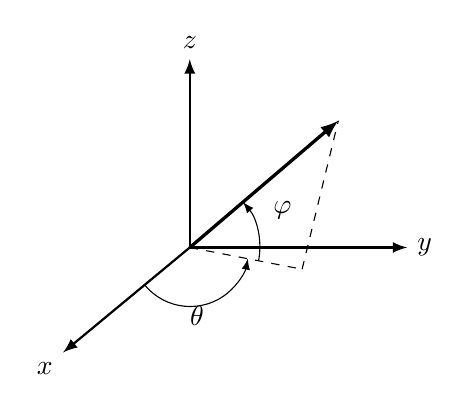
\begin{tikzpicture}[scale=0.92,>=latex]
  \coordinate (O) at (0,0);
  \draw[->,thick] (O) -- (0,2.6) node[above]{$z$};
  \draw[->,thick] (O) -- (3.0,0) node[right]{$y$};
  \draw[->,thick] (O) -- (-1.75,-1.45) node[below left]{$x$};
  \coordinate (V) at (2.05,1.75);
  \coordinate (Q) at (1.55,-0.30);
  \draw[->,very thick] (O) -- (V);
  \draw[dashed] (O) -- (Q);
  \draw[dashed] (Q) -- (V);
  \draw[->] (0.95,-0.18) arc (-10.5:40.5:0.97);
  \node at (1.28,0.52) {$\varphi$};
  \draw[->] (-0.62,-0.52) arc (219.5:349.5:0.81);
  \node at (0.10,-0.95) {$\theta$};
\end{tikzpicture}
\end{minipage}

\vspace{6pt}
\section*{1.\ \ 從 WP 中心到極尖}

\[
\eo(\varphi,\theta)=
\begin{bmatrix}\cos\varphi\cos\theta\\[1pt] \cos\varphi\sin\theta\\[1pt] \sin\varphi\end{bmatrix}
\qquad
\varphi_1=\begin{cases} +35.2644^\circ & \text{上磁極}\\[2pt] -35.2644^\circ & \text{下磁極}\end{cases}
\]

$\eo$ 用 $\varphi_1$、$\et$ 用 $\varphi_2$，兩者不是同一個值。

\section*{2.\ \ 從極尖到指定位置}

\[
\et(\varphi,\theta)=
\begin{bmatrix}\cos\varphi\cos\theta\\[1pt] \cos\varphi\sin\theta\\[1pt] \sin\varphi\end{bmatrix}
\qquad
\varphi_2=\begin{cases} 36.5895^\circ & \text{上磁極}\\[2pt] 0^\circ & \text{下磁極}\end{cases}
\]

\section*{3.}

\noindent\begin{minipage}{\textwidth}
\textbf{(1)\ \ 上磁極}

\begin{minipage}[c]{0.20\textwidth}
\centering
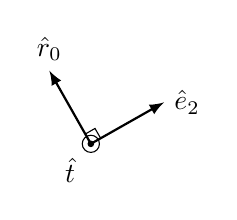
\begin{tikzpicture}[scale=0.62,>=latex]
  \coordinate (O) at (0,0);
  \draw[->,thick] (O) -- (1.5,0.85) node[right]{$\et$};
  \draw[->,thick] (O) -- (-0.85,1.5) node[above]{$\rz$};
  \draw (0.20,0.115) -- (0.085,0.315) -- (-0.115,0.20);
  \filldraw (O) circle (1.6pt);
  \draw (O) circle (5pt);
  \node[below left] at (-0.12,-0.10) {$\tv$};
\end{tikzpicture}
\end{minipage}
\begin{minipage}[c]{0.78\textwidth}
\[
\rz(\varphi,\theta)=\et(\varphi+90^\circ,\theta)=
\begin{bmatrix}-\sin\varphi\cos\theta\\[1pt] -\sin\varphi\sin\theta\\[1pt] \cos\varphi\end{bmatrix},
\qquad \tv=\et\times\rz
\]
\end{minipage}
\end{minipage}

\vspace{6pt}
\noindent\begin{minipage}{\textwidth}
\textbf{(2)\ \ 下磁極}

\begin{minipage}[c]{0.20\textwidth}
\centering
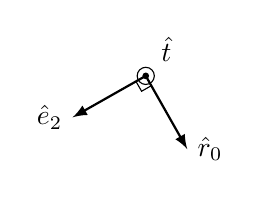
\begin{tikzpicture}[scale=0.62,>=latex]
  \coordinate (P) at (0,0);
  \draw[->,thick] (P) -- (-1.5,-0.85) node[left]{$\et$};
  \draw[->,thick] (P) -- (0.85,-1.5) node[right]{$\rz$};
  \draw (-0.20,-0.115) -- (-0.085,-0.315) -- (0.115,-0.20);
  \filldraw (P) circle (1.6pt);
  \draw (P) circle (5pt);
  \node[above right] at (0.12,0.10) {$\tv$};
\end{tikzpicture}
\end{minipage}
\begin{minipage}[c]{0.78\textwidth}
\[
\rz(\varphi,\theta)=\et(\varphi-90^\circ,\theta)=
\begin{bmatrix}\sin\varphi\cos\theta\\[1pt] \sin\varphi\sin\theta\\[1pt] -\cos\varphi\end{bmatrix},
\qquad \tv=\et\times\rz
\]
\end{minipage}
\end{minipage}

\vspace{8pt}
\textbf{(3)}\quad
$\displaystyle \rh(\alpha,\varphi,\theta)=\cos\alpha\cdot\rz+\sin\alpha\cdot\tv
\qquad
\left\{\begin{aligned}
&\text{上磁極}\ \ \alpha=[0^\circ,\ 360^\circ]\\
&\text{下磁極}\ \ \alpha=[-90^\circ,\ 90^\circ]
\end{aligned}\right.$

\section*{4.}

\[
\nh=\et(\varphi+90^\circ+\beta,\ \theta)\ \ (\text{上極}),
\qquad
\nh=\et(\varphi-90^\circ-\beta,\ \theta)\ \ (\text{下極})
\]
\[
\Longrightarrow\quad
\nh(\alpha,\varphi,\theta)=\cos\beta\cdot\rh(\alpha,\varphi,\theta)-\sin\beta\cdot\et(\varphi,\theta)
\]

\section*{5.\ \ 底面位置}

\textbf{(1)\ \ 上極}
\begin{align*}
\vec{P}_{\text{(mm)}}=\ &0.5\cdot\eo(\varphi,\theta)
+\big[L\cos\beta\big]\,\et(\varphi,\theta)\\[2pt]
&+\big[0.03922+(L-0.03198)\sin\beta\big]\cdot\rh(\alpha,\varphi,\theta)
+0.41\cdot\nh
\end{align*}

\vspace{2pt}
\textbf{(2)\ \ 下極}
\begin{align*}
\vec{P}_{\text{(mm)}}=\ &0.5\cdot\eo(\varphi,\theta)
+\big[L\cos\beta\big]\,\et(\varphi,\theta)\\[2pt]
&+\big[0.03922+(L-0.03280)\sin\beta\big]\cdot\rh(\alpha,\varphi,\theta)
+0.41\cdot\nh
\end{align*}

\end{document}
